\documentclass[fontsize=12pt]{scrartcl} % A4 paper and 11pt font size
\usepackage[a4paper,margin=2cm,bottom=3cm]{geometry}
\usepackage[utf8]{inputenc} % for french
\usepackage[T1]{fontenc} % Use 8-bit encoding that has 256 glyphs
\usepackage[francais]{babel} % English language/hyphenation
\usepackage{amsmath,amsfonts,amsthm} % Math packages
\usepackage{amssymb}
\usepackage{url}

\usepackage{float}
\usepackage{graphicx}

\usepackage{listings}
\usepackage{courier}

\usepackage{wrapfig}

% parameters for listings
\usepackage{color}
\definecolor{mygrey}{rgb}{0.96,0.96,0.96}
\lstset{
  tabsize=4,
  basicstyle=\ttfamily,
  backgroundcolor=\color{mygrey},
  captionpos=b,
  breaklines=true
}

%\fontsize{16pt}

\usepackage{lipsum} % Used for inserting dummy 'Lorem ipsum' text into the template
\usepackage{hyperref}

\usepackage{sectsty} % Allows customizing section commands
\allsectionsfont{\centering \normalfont\scshape} % Make all sections centered, the default font and small caps

\usepackage{eurosym}

\usepackage{fancyhdr} % Custom headers and footers
\pagestyle{fancyplain} % Makes all pages in the document conform to the custom headers and footers
\fancyhead{} % No page header - if you want one, create it in the same way as the footers below
\fancyfoot[L]{} % Empty left footer
\fancyfoot[R]{} % Empty center footer
\fancyfoot[C]{\thepage} % Page numbering for right footer
\renewcommand{\headrulewidth}{0pt} % Remove header underlines
\renewcommand{\footrulewidth}{0pt} % Remove footer underlines
\setlength{\headheight}{13.6pt} % Customize the height of the header

\numberwithin{equation}{section} % Number equations within sections (i.e. 1.1, 1.2, 2.1, 2.2 instead of 1, 2, 3, 4)
%\numberwithin{figure}{section} % Number figures within sections (i.e. 1.1, 1.2, 2.1, 2.2 instead of 1, 2, 3, 4)
\numberwithin{table}{section} % Number tables within sections (i.e. 1.1, 1.2, 2.1, 2.2 instead of 1, 2, 3, 4)

\setlength\parindent{2em} % Removes all indentation from paragraphs - comment this line for an assignment with lots of text
%\setlength{\parskip}{1em}

%\renewcommand{\baselinestretch}{1.5}

%----------------------------------------------------------------------------------------
%	TITLE SECTION
%----------------------------------------------------------------------------------------

\newcommand{\horrule}[1]{\rule{\linewidth}{#1}} % Create horizontal rule command with 1 argument of height

\title{	
\normalfont \normalsize 
\textsc{UJM (Saint-Étienne) // GRAME-CNCM (Lyon) // Gipsa-Lab (Grenoble) // ARCAN (Grenoble)} \\ [25pt] % Your university, school and/or department name(s)
\horrule{0.5pt} \\[0.4cm] % Thin top horizontal rule
\huge 18\textsuperscript{ème} Conférence Sound and Music Computing (SMC-22)\\Saint-Étienne -- Juin 2022\\--------\\\textit{Music Technology and Design} \\ % The assignment title
\horrule{2pt} \\[0.5cm] % Thick bottom horizontal rule
}

\date{} % Today's date or a custom date

\begin{document}

\maketitle % Print the title

\tableofcontents  

\section{La conférence SMC}

Que ce soit dans nos smartphones, nos ordinateurs, nos téléviseurs, nos voitures, dans la musique que l'on écoute (qu'elle soit enregistrée ou lors de concerts), etc., les \textbf{technologies du son, de l'acoustique et de la musique} sont omniprésentes dans nos vies. L'émergence de nouvelles plateformes en lien avec ces domaines (ex. \textbf{réalité virtuelle/augmentée}, \textbf{Intelligences Artificielles (IA)}, \textbf{web apps}, etc.) les placent au centre des développements actuels poussés par les géants du secteur (ex. Facebook, Google, Apple, etc.). L'informatique musicale et la création en musique contemporaine/expérimentale ont longtemps servi d'incubateur pour ces développements et s'en sont nourris. De plus, comme le souligne Ge WANG\footnote{WANG, Ge, Artful Design: Technology in Search of the Sublime, A MusiComic Manifesto, Stanford : Stanford University Press, 2018.}, le design a joué un rôle prépondérant dans ces développements, plaçant ce domaine au centre de préoccupations Stéphanoises. 

De manière plus précise, le calcul du son et de la musique (SMC -- \textit{Sound and Music Computing}) est un domaine de recherche dont le but est d'étudier les liens entre musique, acoustique et technologie d'un point de vue interdisciplinaire. SMC peut être découplé en un ensemble de sous-domaines comprenant :

\begin{itemize}
  \item \textbf{le traitement des signaux audio/acoustiques et musicaux} qui regroupe l'ensemble des techniques de traitement du signal pour l'analyse, la synthèse et la transformation des signaux musicaux et audio ;
  \item \textbf{la compréhension et la modélisation des sons et de la musique} qui regroupent la musicologie computationnelle, la récupération automatisée d'informations musicales et l'aspect informatique des sciences cognitives appliquées à la musique ;
  \item \textbf{les interfaces pour le contrôle du son et de la musique} qui sont directement liées au domaine des Interfaces Homme/Machine (IHM) ;
  \item \textbf{l'assistance à la création musicale et sonore} qui regroupe le design sonore, les langages de programmation associés à ce domaine et la composition assistée par ordinateur.
\end{itemize}

La conférence SMC (\textit{Sound and Music Computing}) a été fondée en 2004 et est le fruit de l'union des JIMs (\textit{Journées de l'Informatique Musicale})\footnote{\url{http://jim.afim-asso.org/}} française et de leur équivalent italien : les CIMs (\textit{Colloqui di Infromatica Musicale})\footnote{\url{http://www.aimi-musica.org/}}. SMC a depuis pris une ampleur considérable pour devenir une plateforme d'échange internationale pluridisciplinaire à la croisée des arts, des sciences et des nouvelles technologies, rendez-vous incontournable des communautés de traitement du signal audio, des interfaces homme/machine pour la musique, de l'informatique musicale, des sciences cognitives appliquées à la musique, etc. SMC a lieu chaque année dans une grande ville européenne (ex. Málaga, Chypre, Helsinki, Hambourg, Dublin, Athènes, etc. pour les six dernières éditions) et \textbf{réunit des conférenciers et des artistes venant des quatre coins du monde}.

SMC s'organise traditionnellement autour de trois grands évènements : \textbf{une école d'été} (\textit{Summer School}), \textbf{une conférence scientifique} et \textbf{un programme artistique} riche et varié avec des \textbf{concerts} et des \textbf{installations/expositions}. L'édition Stéphanoise de SMC sera également complétée d'\textbf{une série d'évènements autour de la médiations et de la transmission s'adressant au grand public} (scolaires, particuliers, etc.) ainsi que d'\textbf{un salon des technologies de l'audio et de la musique} lors duquel les entreprises du notre domaines pourront exposer leurs produits. 

\begin{figure}[h]
  \centering
  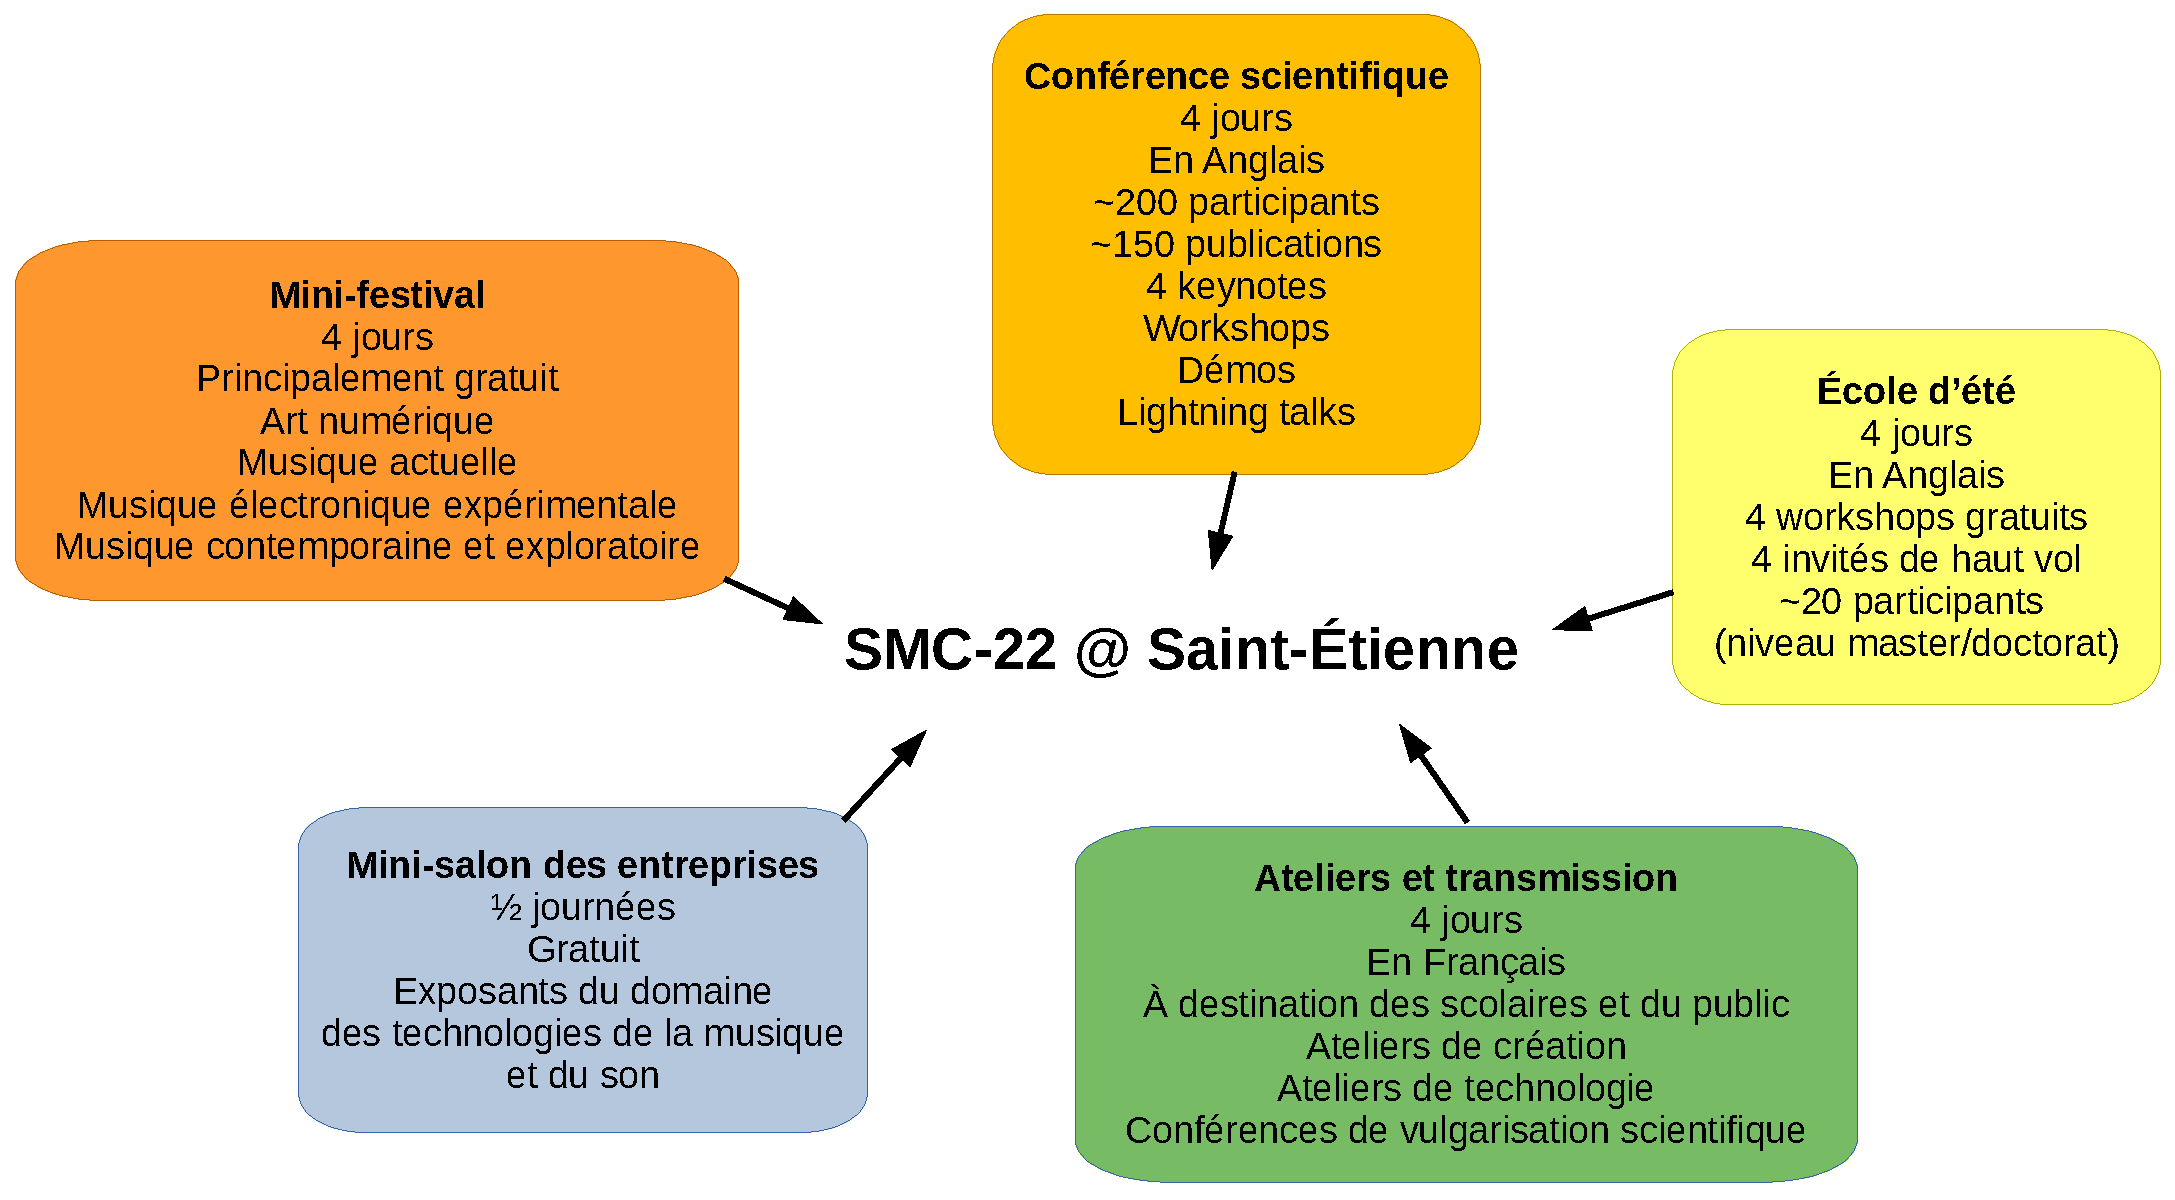
\includegraphics[width=\columnwidth]{img/overview}
  \caption{SMC-22 à Saint-Étienne}
  \label{fig:overview}
\end{figure}

\section{SMC à Saint-Étienne : un évènement art/science tourné vers le grand public}

\textbf{Décloisonnement, transversalité et transdisciplinarité} sont devenus les maîtres mots de la création et de la vie culturelle. Les schémas institutionnels antérieurs à cette révolution sont bouleversés. Il faut \textbf{inventer les modèles culturels du futur}. Cette époque est à ce titre passionnante, remplie d'enjeux, de questions, de pistes de réflexion. De \textbf{nouveaux lieux et évènements}, partout dans le monde, dans toutes les grandes métropoles, tentent aujourd'hui de réinventer la notion d'espace culturel, de lieu social de partage de la création. La \textbf{modularité, la réactivité et la connectivité} sont les clés de ces nouvelles plateformes. Et plus encore la capacité à capter la rapidité et l'effervescence de l'époque. 

L'édition stéphanoise de SMC s'inscrit dans ce contexte et se veut être une \textbf{plateforme d'échange entre scientifiques, artistes de tous bords, industriels, scolaires et grand public}. En plus de cette volonté d'ouverture, SMC-22 mettra l'accent sur \textbf{le design et les nouvelles technologies} en ayant pour thème : \textbf{Music Technology and Design} (technologie de la musique et design). Nous souhaitons que cet évènement \textbf{touche le public Stéphanois de la manière la plus large possible} à travers un ensemble d'\textbf{évènements gratuits} annexes à la conférence à destination du grand public : 

\begin{itemize}
\item \textbf{concerts et installations} autour des \textbf{arts numériques} et de la \textbf{musique actuelle},
\item \textbf{ateliers pour les scolaires et le public},
\end{itemize}

Pour cela, nous nous appuierons sur l'expérience du GRAME-CNCM\footnote{\url{http://www.grame.fr}} et de l'association ARCAN\footnote{\url{http://www.arcan.io/}} dans les domaines de l'organisation de festivals et de la médiation/transmission (cf. \S\ref{sec:part}).  

\subsection{École d'été}
\label{subsec:summerSchool}

L'école d'été de SMC aura lieu pendant quatre jours juste avant le début de la conférence. Elle se composera d'\textbf{une série de workshops} (en Anglais) d'une journée sur des \textbf{sujets de pointe} à destination d'\textbf{étudiants internationaux au profil d'excellence} en master ou en doctorat. Elle aura pour thème : \textbf{technologie de la musique et design}.

Les intervenants suivants sont pré-sentis pour intervenir lors de l'école d'été de SMC\footnote{Cette liste n'est pas arrêtées.} :

\begin{itemize}
  \item \textbf{Ge WANG} -- professeur à l'école de design (D-School) et au Center for Computer Research in Music and Acoustics (CCRMA) de l'université Stanford, co-fondateur de la startup Smule, auteur de \textit{Artful Design: Technology in Search of the Sublime, A MusiComic Manifesto} ;
  \item \textbf{François PACHET} -- directeur du Spotify Creator Technology Research Lab, auteur de \textit{Deep Learning Techniques for Music Generation}, producteur d'\textit{Hello World}, le premier album de musique intégralement composé par une intelligence artificielle ;
  \item \textbf{Yann ORLAREY} -- directeur scientifique de GRAME-CNCM, inventeur du langage de programmation Faust ;
  \item \textbf{Roger LINN} -- fondateur de Roger Linn Design, inventeur de la boîte à rythme et du \textit{LinnStrument} récompensé par une Grammy Award.
\end{itemize} 

Nous pensons limiter l'école d'été à une \textbf{vingtaine de participants}. Son inscription ne sera \textbf{pas payante}. \textbf{Huit places seront réservées à des étudiants Stéphanois}. 

\subsection{Conférence scientifique}

D'une durée de \textbf{quatre jours}, la conférence scientifique fait suite à l'école d'été de SMC. \textbf{Entre 150 et 200 personnes} y participent. De la \textbf{volonté d'ouverture et de la nécessité d'invention de modèles nouveaux}, notamment au titre de la \textbf{médiation et de la culture scientifique}, les organisateurs de cette édition de SMC souhaitent \textbf{sortir des formes conventionnelles} de ce type de rencontres. Tout d'abord, en proposant cinq types de présentations: \textbf{posters}, \textbf{lightning talks}, \textbf{keynotes}, \textbf{démonstrations} et \textbf{workshops}. Ensuite, en jouant littéralement le décloisonnement et en rompant avec les lieux ``sanctuaires'' et souvent hermétiques de la production et diffusion scientifique, afin de s'inviter au cœur de lieux de vie et de Culture de la ville de Saint-Étienne.

\paragraph{\textbf{Posters}} L'ensemble des contributions scientifiques de la conférence sont présentées sous la forme de posters. Chaque poster fait l'objet d'une publication dans un article publié aux termes de la conférence dans les actes (\textit{proceedings}). La sélection des contributions est effectuée par un commité international d'experts dirigé par le président scientifique de la conférence (\textit{paper chair}). Une quinzaine de posters sont présentés à chaque session. Les sessions débutes par une première phase (appelée \textit{poster craze}) où les auteurs de chaque contribution présentent le contenu de leur poster sous la forme de courtes présentations d'une minute trente. Lors d'une seconde phase (d'une durée d'une heure), les intervenants tiennent des ``stands'' où leur poster est affiché et où ils peuvent interagir avec les participants de la conférence. Les conférenciers sont alors libres de circuler dans la pièce. Un buffet avec des rafraîchissements et des snacks est mis à leur disposition lors de cette période. Une quinzaine de sessions de ce type auront lieu pendant SMC-22.

\paragraph{\textbf{Lightning Talks}} Les \textit{lightning talks} sont de présentations de trente minutes faites par des conférenciers. Un total de huit lightning talks (deux par jours) sera donné à SMC-22. À la manière des ``Ted Talks'', ce type de présentation se veut être vivant et ludique. Leur sujet est libre et ne fait pas nécessairement l'objet d'une publication scientifique. Les conférenciers soumettent des proposition de lightning talk en aval de la conférence qui sont ensuite sélectionnés par le commité d'organisation. 

\paragraph{\textbf{Keynote}} Les \textit{keynotes} (conférence plénière) sont des présentations d'une heure faites par des membres reconnus de la communauté scientifique invités à la conférence. Quatre keynotes seront donnés lors de SMC-22 par les intervenants de l'école d'été : Ge WANG, Roger LINN, Yann ORLAREY et François PACHET (voir \S\ref{subsec:summerSchool}).

\paragraph{\textbf{Démos}} Les démos permettent de présenter des outils/des technologies en interagissant directement avec le public. Les sessions de démos prennent la même forme que les sessions de posters : les démonstrateurs tiennent des ``stands'' dans une grande pièce où le public peut circuler. À la différence des posters, les démos sont sélectionnées directement par le comité d'organisation de la conférence.

\paragraph{\textbf{Workshops}} D'une durée de deux heures, les workshops sont des ateliers/cours lors desquels des outils ou des technologies de pointe sont présentés aux participants. Le nombre de participants à un workshop est limité (en général 30 personnes sauf recommandation particulière de l'intervenant). Les workshops sont sélectionnés directement par le comité d'organisation de la conférence.\\

SMC étant une conférence de type ``single track'', les sessions n'ont jamais lieu en parallèle, sauf pour les workshops. Un maximum de deux workshops aura lieu en même temps. Les sessions de présentations orales sont généralement entrecoupées de pauses café. De la même manière, l'inscription à la conférence comprend généralement les déjeuners. La conférence est payante pour les conférenciers (les personnes présentant leurs travaux). Les frais d'inscription n'ont pas encore été fixés mais ils sont généralement d'environ 400\euro{} pour le plein tarif et 250\euro{} pour les étudiants. Toutefois, afin de rendre SMC-22 accessible au plus grand nombre, \textbf{nous souhaitons que la conférence soit ouverte gratuitement aux auditeurs libres}.

\subsection{Mini-festival: programme artistique} 

\textbf{Un programme artistique riche et varié centré autour des nouvelles technologies} aura lieu en parallèle de la conférence, prenant la forme d'un ``mini-festival.'' Nous souhaitons organiser plusieurs concerts (au moins deux par jours) \textbf{gratuits} en fin d'après-midi/soirée et mettre en place des \textbf{installations interactives} durant les quatre jours de la conférence dans différents lieux de la ville. 

Pour cette édition Stéphanoise, nous souhaitons mettre l'\textbf{accent sur les arts numériques et les musiques actuelles} pour toucher un public le plus large possible. Ainsi, les œuvres jouées lors de SMC-22 pourront être classées dans la catégories suivantes :

\begin{itemize}
  \item installations interactives,
  \item performances d'art numérique,
  \item musique actuelle (électro, techno, rock, etc.),
  \item musique électronique expérimentale,
  \item musique contemporaine et exploratoire. 
\end{itemize} 

Pour se faire, nous nous appuierons sur l'expertise et le savoir faire de GRAME-CNCM et de l'association ARCAN dans l'organisation de ce type d'évènement (cf. \S\ref{sec:part}).

Deux appels à candidature pour participer au mini-festival de SMC en tant qu'artiste seront lancés : 

\begin{itemize}
  \item un appel international en Anglais visant les membres de la communauté SMC et piloté par le commité musical international de la conférence et son président (music chair),
  \item un appel local/national en Français visant les membres de la communauté des arts numériques en France et géré par l'association ARCAN.
\end{itemize} 

En parallèle de ces deux appels, le GRAME-CNCM, l'association ARCAN, le commité d'organisation de la conférence, ainsi que les partenaires musicaux stéphanois de SMC-22 comme le FIL se réserveront le droit de programmer des artistes de leur choix. 

À l'heure actuelle, nous savons que certains de ces concerts pourront avoir lieu au FIL (performances d'art numérique et musique actuelle) qui est partenaire de SMC-22 et à la maison de l'université sur le campus Tréfilerie. Nous sommes à la recherche d'autres lieux pour étendre cette action à l'échelle de toute la ville. 

Tandis que la conférence scientifique de SMC-22 s'adressera à un public de spécialistes, \textbf{ce ``mini-festival'' constituera, avec nos actions de médiations et de transmission la partie visible de cet évènement pour le grand public}.

\subsection{Action de médiation et transmission vers le grand public}

Le domaine des technologies de l'audio et de la musique irradie complètement notre société à l'ère du numérique. La plupart des objets que nous utilisons dans notre vie courante produisent du son (ex. smartphones, assistants personnels, voitures, télévisions, casques, haut-parleurs, etc.) et des technologies de pointe se trouvent derrière tous ces objets. La formation et la sensibilisation du grand public et des futurs générations à ces questions est un enjeux stratégique de société et de compétitivité à l'échelle internationale. De la même manière, l'art jouant un rôle de caisse de resonance de notre société, les pratiques artistiques qui découlent de ces innovations doivent être valorisées. % C'est un peu fumeux ça.

Le département de transmission de GRAME-CNCM sous la direction de Catinca DUMITRASCU organise des actions de médiation dans ce sens depuis plusieurs années (cf. \S\ref{sec:part}). Dans le cadre de SMC-22, nous mettrons en avant des projets de médiation portés par le GRAME tels que \textbf{Smartmômes} (cf. \S\ref{app:smartmomes}), \textbf{AmStramGrame} (cf. \S\ref{app:amstram}), \textbf{Light Wall System} (cf. \S\ref{app:lightwall}), \textbf{Airmachine} (cf. \S\ref{app:airmachine}), \textbf{Marathon créatif} (cf. \S\ref{app:marathon}), \textbf{Massages sonores} (cf. 
\S\ref{app:massage}), \textbf{Vibes} (cf. \S\ref{app:vibes}), \textbf{Veggie Orchestra} (cf. \S\ref{app:veggie}), etc. et nous organiserons \textbf{une série d'atelier grand public} sur des sujets allant du design sonore au lutherie numérique en passant par la programmation informatique, etc. ainsi que des \textbf{conférences de vulgarisation scientifique} en Français pour le public Stéphanois.

\paragraph{\textbf{AmStramGrame}} AmStramGrame (cf. \S\ref{app:amstram}) est un projet art/science porté par GRAME-CNCM et réseau canopé\footnote{\url{https://www.reseau-canope.fr/}} (éducation nationale). Il vise à faciliter l'apprentissage des matières scientifiques telles que les mathématiques et la physique par la programmation d'instruments de musique modulaires et portables appelés \textit{Gramophone} (cf. figure~\ref{fig:gramo}). Une fois programmé, un travail est effectué avec des artistes pour les utiliser dans un contexte musical. \textbf{Des ateliers AmStramGrame seront organisés dans les lycées et collège de la région au cours de l'année 2022}. SMC-22 pourrait servir de temps fort en permettant aux élèves de \textbf{présenter leur travail lors d'un concert}. En parallèle, nous souhaiterions organiser des ateliers AmStramGrame pour le grand public pendant les 4 jours de la conférence. Ces derniers pourraient \textbf{avoir lieu en extérieur sur une place de Saint-Étienne} (Jean Jaurès ?). Les badauds pourraient alors apprendre des concepts de base de programmation informatique et de synthèse de son dans le but de créer leur propre instrument de musique au travers du Gramophone. \textbf{Des performances ponctuelles pourraient avoir lieu sur la place lors de ces ateliers}.  

\begin{figure}[h]
  \centering
  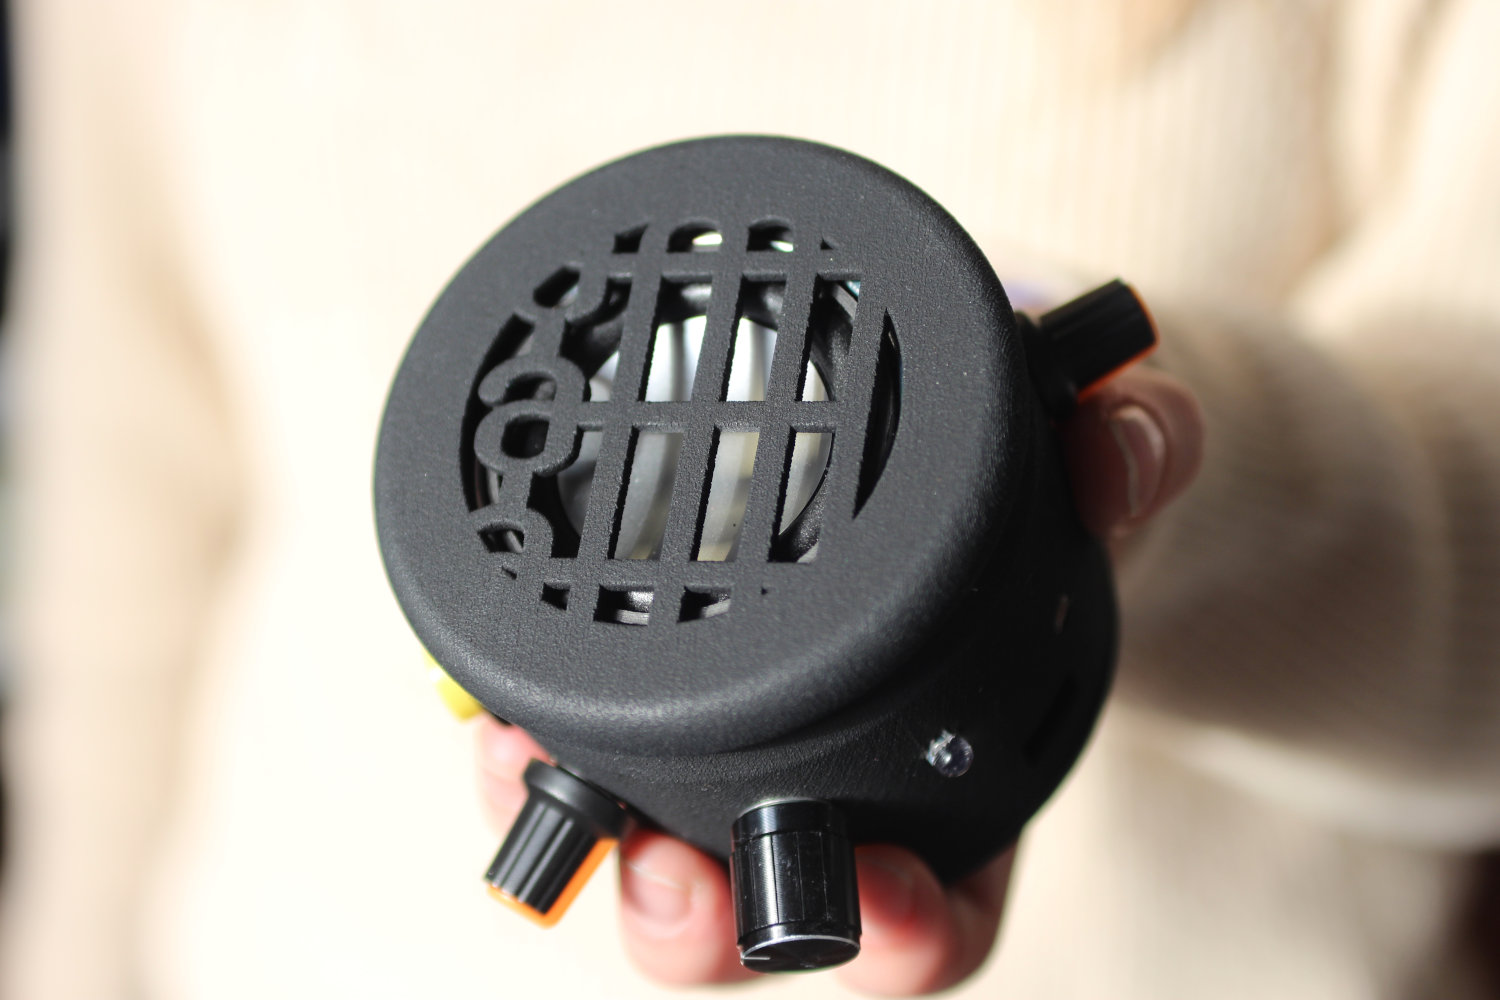
\includegraphics[width=12cm]{img/gramo}
  \caption{Le Gramophone utilisé lors des ateliers AmStramGrame}
  \label{fig:gramo}
\end{figure}

\paragraph{\textbf{Ateliers}} En plus d'AmStramGrame qui est actuellement le projet phare du département de transmission de Grame, nous souhaitons organiser des ateliers autour des autres projets portés par cette structure à déstination du grand public et des scolaires tel que \textbf{Smartmômes} (cf. \S\ref{app:smartmomes}), \textbf{Light Wall System} (cf. \S\ref{app:lightwall}), \textbf{Airmachine} (cf. \S\ref{app:airmachine}), \textbf{Marathon créatif} (cf. \S\ref{app:marathon}), \textbf{Massages sonores} (cf. 
\S\ref{app:massage}), \textbf{Vibes} (cf. \S\ref{app:vibes}) et \textbf{Veggie Orchestra} (cf. \S\ref{app:veggie}).

\paragraph{\textbf{Conférences grand public}} À la fin de chaque journée de SMC-22, \textbf{une conférence gratuite grand public en Français de vulgarisation scientifique sera proposée}. Les conférenciers de SMC-22 auront la possibilité de proposer des sujets de conférence de ce type sur le site internet de SMC-22. Le sujet de ces conférences sera choisi par les organisateur parmi les propositions.

\subsection{Mini-salon des entreprises}

Notre domaine, en étant à la pointe de l'innovation, a toujours entretenu un lien fort avec des entreprises de tous bords (spécialisées et plus généralistes) tel que Yamaha, Arturia, Ableton, Apple, Google, Tesla, Roli, etc. et plus récemment ExpresiveE, HyVibe, Antescofo, etc. Des ingénieurs de ces sociétés se rendent d'ailleurs chaque années à SMC en tant qu'auditeurs libres pour être au fait des derniers développement dans le milieu de la recherche. \textbf{Nous souhaitons mettre en valeur les technologies développées dans l'industrie lors de cette édition Stéphanoise de SMC en offrant la possibilité à des entreprises de venir exposer leurs produits lors d'un ``mini-salon''} qui aura lieu pendant une demie journée en parallèle de la conférence scientifique.   

\subsection{Événements annexes}

SMC-22 est l'opportunité de faire connaître le patrimoine culturel de Saint-Étienne et de ses environs à notre communauté scientifique et artistique. 

Le banquet de SMC-22 a généralement lieu le soir du troisième jour de la conférence. Pour cette édition Stéphanoise, nous souhaiterions qu'un groupe de musique traditionnelle local anime la soirée.

Nous souhaitons également organiser des visites touristiques de Saint-Étienne et de ses alentours pour les conférenciers.

\section{Partenaires, organisateurs et comités scientifiques et artistiques}
\label{sec:part}

L'organisation de SMC-22 est le fruit d'une collaboration entre le \textbf{CIEREC}\footnote{\url{https://www.univ-st-etienne.fr/fr/cierec.html}} (\textit{Centre Interdisciplinaire d'Études et de Recherches sur l'Expression Contemporaine}) de l'\textbf{université Jean Monnet de Saint-Étienne}, le \textbf{GRAME-CNCM}\footnote{\url{http://www.grame.fr}} (\textit{Centre National de Création Musicale}) de Lyon, le \textbf{Gipsa-Lab}\footnote{\url{http://www.gipsa-lab.fr}} de l'institut polytechnique de Grenoble, l'association \textbf{ARCAN}\footnote{\url{http://www.arcan.io/}}, ainsi que d'un grand nombre d'autres partenaires :

\begin{itemize}
\item le \textbf{FIL -- scène de musique actuelle} : \url{http://www.le-fil.com} ;
\item l'\textbf{INSA} (\textit{Institut National des Sciences Appliquées}) Lyon: \url{https://www.insa-lyon.fr} ;
\item l'\textbf{université de Lyon} : \url{https://www.universite-lyon.fr/}
\item l'\textbf{INRIA} : \url{https://www.inria.fr/}
\item le \textbf{CCRMA} (\textit{Center for Computer Research in Music and Acoustics}) de l'\textbf{université Stanford} : \url{https://ccrma.stanford.edu/~rmichon}
\item et bien d'autres d'ici SMC-22 :).
\end{itemize}

Une vue d'ensemble des membres du comité d'organisation de SMC-22 est présentée dans le tableau suivant :

\begin{table}[!htbp]
  \begin{center}
    \begin{tabular}{c | c}
      \textbf{Nom} & \textbf{Role} \\
      \hline
      \hline
      Romain MICHON & organisateur/président (Principal Chair) \\
      Laurent POTTIER & organisateur/président (Principal Chair) \\
      Yann ORLAREY & président du comité scientifique (Paper Chair) \\
      Constantin BASICA & président du comité artistique (Music Chair) \\
      Jérôme VILLENEUVE & programmation artistique et direction technique \\
      James LEONARD & président de l'école d'été (Summer School Chair) \\
      Catinca DUMITRASCU & transmission/médiation/liens avec le public \\
    \end{tabular}
  \end{center}
\end{table}

\paragraph{\textbf{CIEREC}} Le Centre Interdisciplinaire d'Études et de Recherches sur l'Expression Contemporaine (CIEREC) est basé sur le campus tréfilerie de l'Université Jean Monnet (UJM) de Saint-Étienne. Il a une grande expérience dans le domaine de l'organisation de conférence autour des technologies de l'audio et de l'informatique musicale (ex. Journées de l'Informatique Musicale 2011, Linux Audio Conference 2017, etc.). Laurent POTTIER et Vincent CICILIATO sont tous les deux enseignant chercheur au CIEREC et directeurs du Master RIM/RAN\footnote{Réalisateur en Informatique Musicale/Art Numérique} et membre du commité d'organisation de SMC-22. 

\paragraph{\textbf{GRAME-CNCM}} Le GRAME-CNCM est un Centre National de Création Musical (label du ministère de la culture) basé à Lyon. Son activité de découple en trois pôles : production, transmission et recherche scientifique. Le Grame organise la ``biennale musique en scène'' qui rassemble des milliers de spectateurs, des concerts, des résidences d'artiste, etc. Il intervient dans les écoles, les collèges et les lycée de la région pour des actions pédagogiques artistiques et de vulgarisation scientifique à travers des projets tel que SmartFaust, LightWall System (cf. \S\ref{app:lightwall}) et plus récemment AmStramGrame (cf. \S\ref{app:amstram}). Les travaux de l'équipe de recherche de Grame sur les systèmes embarqués et les langages de programmations pour l'audio et la musique sont reconnus à l'échelle internationale. Romain MICHON est enseignant-chercheur dans l'équipe de recherche du Grame, Yann ORLAREY en est son directeur scientifique et Catinca DUMITRASCU est la responsable du pôle transmission. Ils font tous les trois partie du commité d'organisation de SMC-22.

\paragraph{\textbf{Gipsa-Lab}} Le Gipsa-Lab (Grenoble Images Parole Signal Automatique) est un laboratoire de l'Université Grenoble Alpes (UGA) abritant une unité de recherche en technologie de l'audio et de la musique à laquelle Jérôme VILLENEUVE et James LEONARD (membres du commité d'organisation de SMC-22) sont tous les deux rattachés.

\paragraph{\textbf{ARCAN}} L'Association Ressource pour la Création Artistique Numérique a pour objet l'activation et la mise en réseau des forces en présence sur son territoire (Auvergne Rhône-Alpes) étant en capacité d'œuvrer à l'évolution et au rayonnement des pratiques de la création artistique numérique. Ressource directe pour les créateurs engagés dans une démarche artistique impliquant l'outil numérique, ARCAN est également porteuse d'actions de diffusion, de médiation et de pédagogie à destination de tous les publics. ARCAN organise le festival DN[A] et Negotium\footnote{\url{http://www.arcan.io/}} qui rassemblent des milliers de participants chaque année autour des arts numériques. DN[A] en particulier mobilise l'ensemble des lieux phare de l'agglomération Grenobloise.

\section{Contacts}

\begin{itemize}
\item Romain Michon, GRAME-CNCM -- \texttt{michon@grame.fr} -- 07 67 39 72 40
\item Laurent Pottier, UJM -- \texttt{laurent.pottier@univ-st-etienne.fr} % -- TODO: tel Laurent ?
\end{itemize}

\section{Un petit mot pour la fin}

Saint-Étienne incarne les valeurs que nous tentons de porter avec cette édition spéciale de SMC : ouverture, dynamisme, innovation, partage, technologie, culture, transmission, etc. Le choix de Saint-Étienne pour organiser SMC-22 n'est pas un hasard. La plupart de nos structures se trouvent dans la région (Lyon, Grenoble, etc.) mais nous croyons profondément au dynamisme de Saint-Étienne et nous pensons qu'un évènement comme SMC est totalement en phase avec les orientations prisent par la ville en direction du design et des nouvelles technologies, entre autre. Nous souhaitons que SMC contribue à renforcer l'image de Saint-Étienne à l'échelle nationale et internationale comme pôle d'innovation, de dynamisme, d'ouverture et de modernité. Nous sommes fiers que SMC ait lieu à Sainté en 2022. 

\pagebreak

\appendix

\section{Smartmômes}
\label{app:smartmomes}

\begin{wrapfigure}{l}{7cm}
\centering
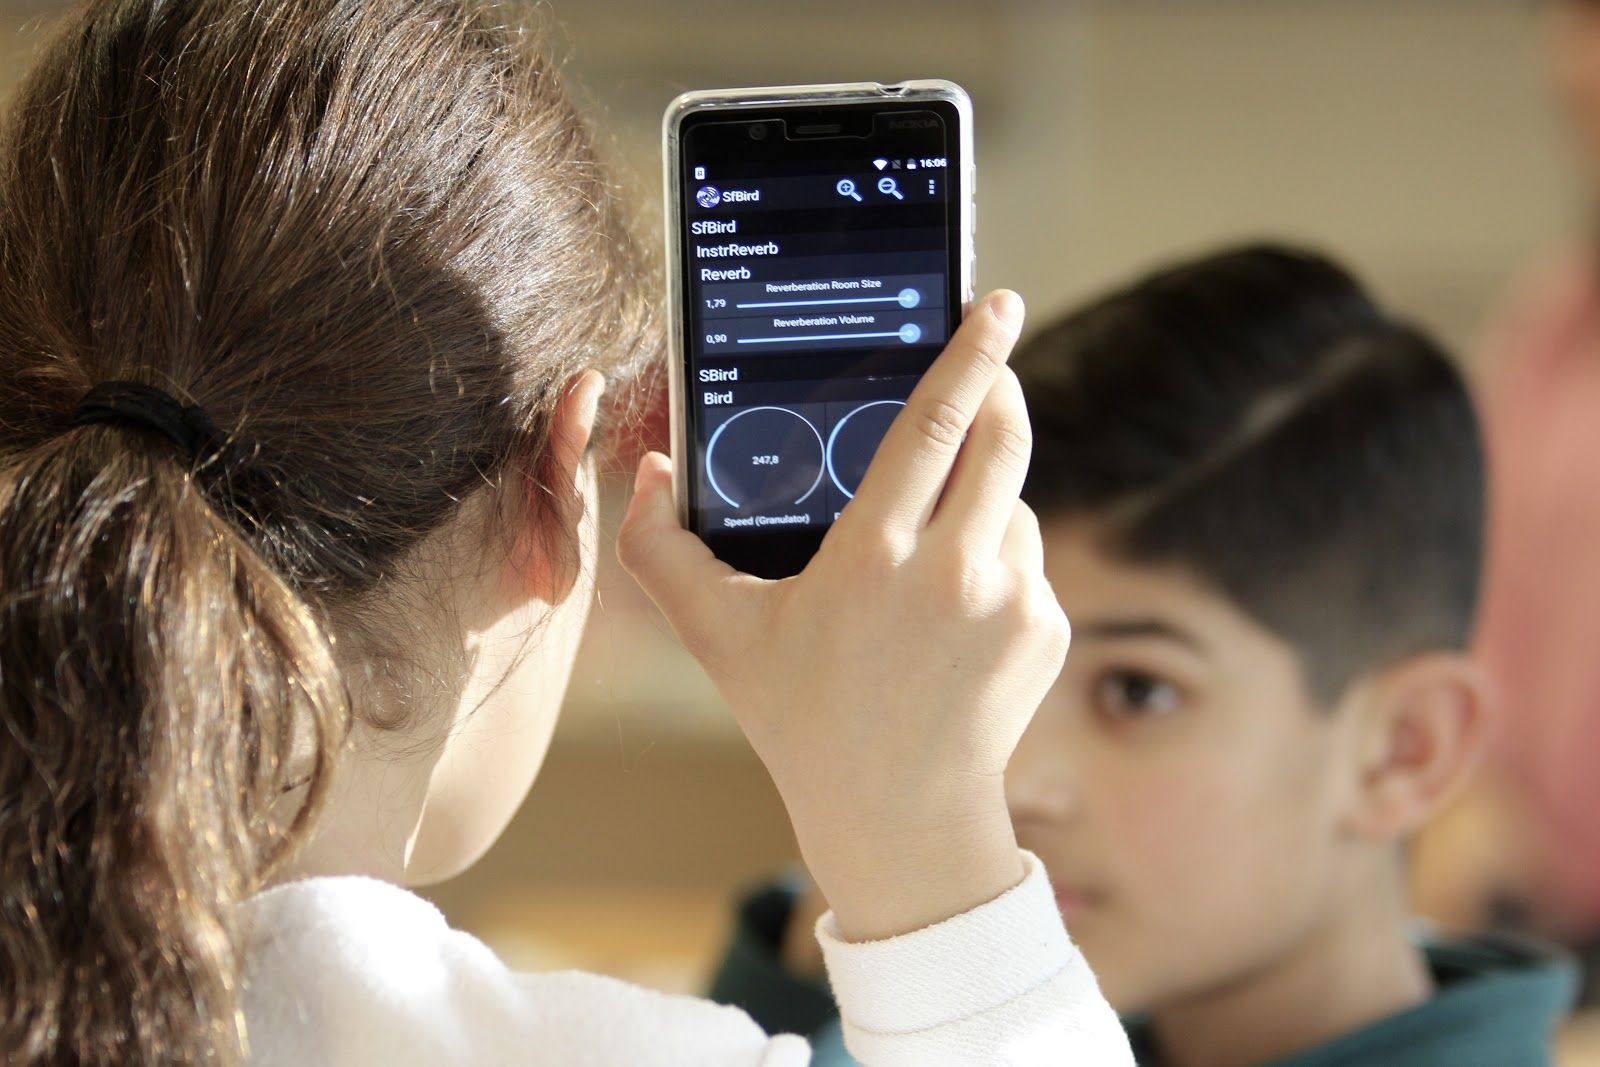
\includegraphics[width=6.5cm]{img/smartmomes}
\label{fig:sm}
\end{wrapfigure}

Détourner un objet omniprésent de notre quotidien pour en faire un instrument de musique, tél est le défi !

Smartmômes est un projet à destination du tout public, porté par Grame depuis 2014, ayant comme support non pas des instruments de musique traditionnels, mais des téléphones portables. Le fil conducteur du projet est le geste musical : c'est en effet le mouvement des téléphones qui génère les sons et non un ``pianotage'' sur l'écran.

Accompagnés par un artiste Grame, les participants sont invités à découvrir les applications musicales pour smartphones intitulées GameLAN.
 
GameLAN est un ensemble d'applications musicales conçues par Grame qui s'appuient sur la technologie Faust\footnote{\url{https://faust.grame.fr}}. Elles ont été imaginées pour êtres jouées en utilisant simplement les mouvements du smartphone. Pas de prérequis musical, seul vos gestes feront de vous un musicien ! Les 7 applications de la famille GameLAN (Attackey, Baliphone, DroneLAN, Sequenceur, ShakerXY, Sinusoïde, Atomicro) peuvent être jouées en solo ou en orchestre.
 
L'atelier est imaginé comme un espace de rencontre questionnant la forme du concert, la posture de l'interprète et son instrument.\\

\noindent
\textbf{Publics :} scolaires dès 8 ans, périscolaires, adultes, personnes âgées ou en situation de handicap. 

\noindent
\textbf{À décliner en atelier scolaire ou tout public}.

\pagebreak

\section{AmStramGrame}
\label{app:amstram}

\begin{wrapfigure}{l}{7cm}
\centering
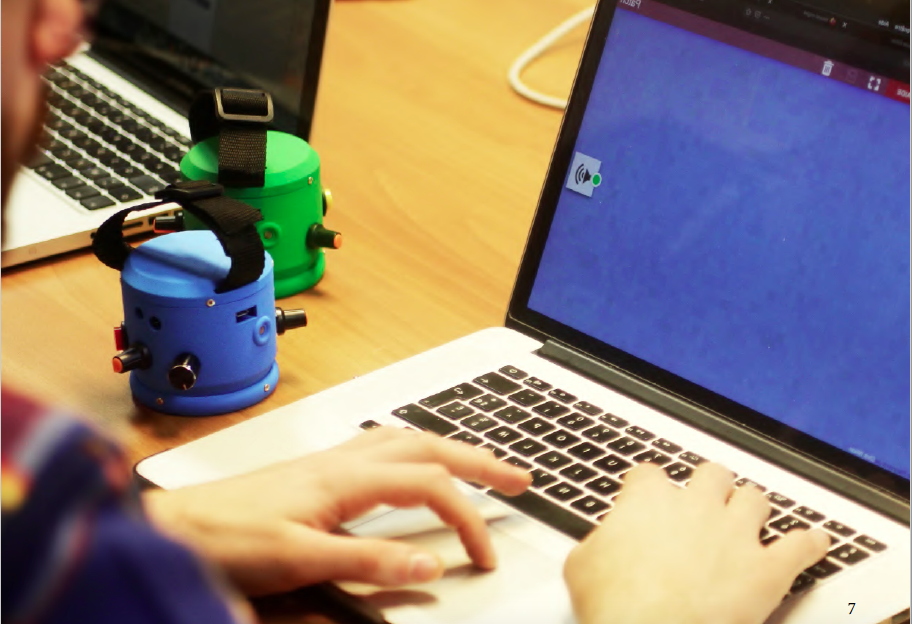
\includegraphics[width=6.5cm]{img/amstram}
\label{fig:amstram}
\end{wrapfigure}

Imaginé par Grame et réseau canopé\footnote{\url{https://www.reseau-canope.fr/}}, Amstramgrame est un projet pédagogique arts et sciences réunissant ateliers et outils à destination de la communauté éducative permettant une mise en application concrète de concepts scientifiques parfois abstraits en utilisant la création sonore et la programmation informatique comme vecteurs.

Le projet s'appuie sur le langage de programmation Faust créé et développé par Grame depuis 15 ans et reconnu comme un standard dans le domaine du traitement du signal en temps réel pour l'audio. 

Les ateliers sont basés sur des scénarii pédagogiques courts et modulables. Chaque atelier a une approche à la fois artistique et scientifique.Le projet nécessite l'utilisation d'ordinateurs pour accéder au site web Amstramgrame, qui permet de construire des instruments de musique électronique en ligne, avec quelques lignes de code, et de programmer les gramophones (instruments audio spécialement conçu pour l'atelier qui réagissent aux gestes de l'utilisateur).
 
Les participants expérimentent ensuite le contrôle gestuel de leurs instruments et imaginent des situations (performances musicales ou dansées, installations) en lien avec la lutherie numérique créée.

AmStramGrame dispose d'une centaine de Gramophones pouvant être facilement déployés sur le terrain.

Ce projet fait actuellement l'objet d'une collaboration avec le FIL, le château du rozier à Feurs (42) et le collège de Feurs autour des lutheries numériques.\\

\noindent
\textbf{Projet adapté à toutes les disciplines (mathématiques, physique, technologie, musique, français, eps, etc.), à tous les niveaux d'âge (du cycle primaire au secondaire) et accessible aussi bien aux élèves inscrits dans un parcours d'enseignement musical, qu'à ceux sans aucun enseignement artistique.}

\noindent 
\textbf{À décliner en atelier scolaire ou tout public.}
 
\noindent 
\textbf{Possibilité d'organiser des ateliers en extérieur.}

\pagebreak

\section{Light Wall System}
\label{app:lightwall}

\begin{wrapfigure}{l}{7cm}
\centering
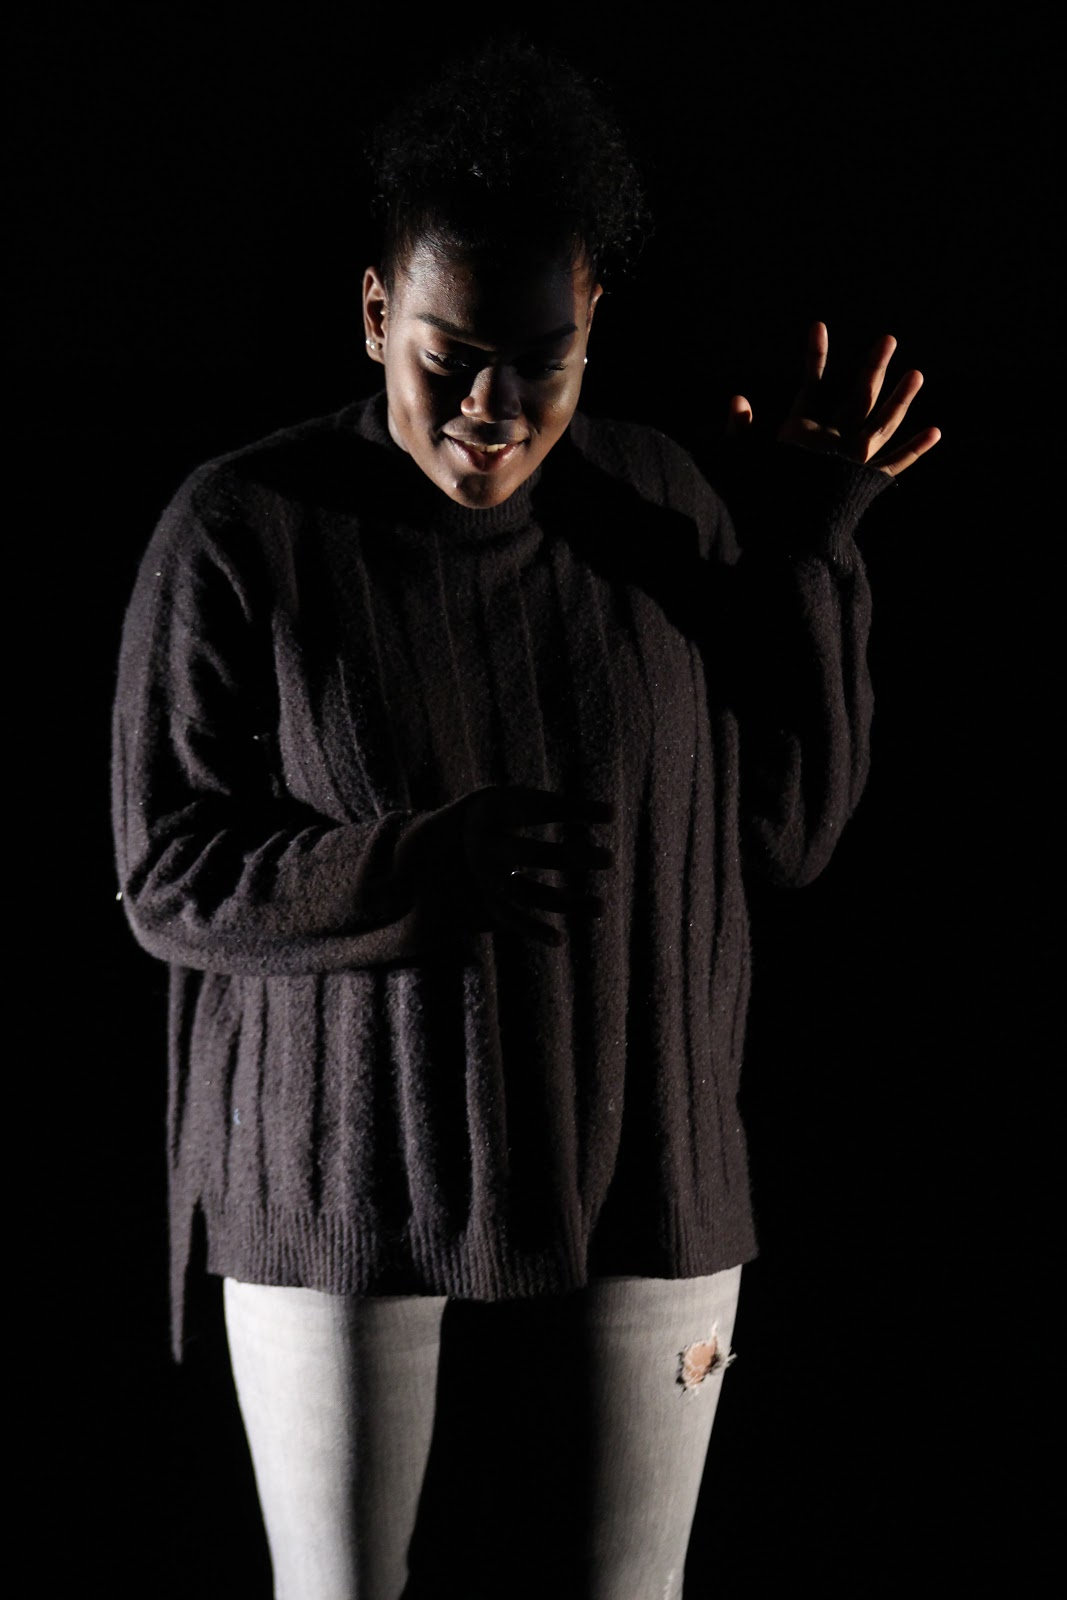
\includegraphics[width=6.5cm]{img/lightwall}
\label{fig:lightwall}
\end{wrapfigure}

Arriver sur scène sans instrument, se placer bien au centre et avancer les bras, les jambes, la tête, le corps dans la lumière\dots Voir son empreinte devant soi et entendre immédiatement un son qui se propage dans l'espace : le son du mouvement, de son propre mouvement, de sa respiration\dots voilà ce que propose \textit{Light Wall System}.

Light Wall System est une interface où l'interprète produit des sons grâce aux déplacements de son corps à travers un faisceau lumineux. Ce mur de lumière fonctionne comme un instrument dont on doit s'approprier la contrainte : moduler un son dans l'espace et pouvoir l'arrêter. Il s'agit avant tout de jouer, au sens propre du terme, de façon intuitive et innée dans la lumière. Jouer des sons comme l'on pourrait peindre sur une toile avec ses mains. Light Wall System permet d'explorer les liens possibles entre musique et danse, son et geste ; il nous oblige à repenser l'espace scénique et la place même de l'interprète sur scène. L'objectif est de permettre aux enfants de se retrouver sur scène autrement.

Avec Light Wall System, l'objectif est, d'une part, de toucher des publics de tout horizon (musiciens, danseurs, chorégraphes, amateurs) et d'autre part de fournir un outil adapté aux pédagogues (de l'enseignement général ou spécialisé) qui pourront créer des situations fondées sur les différentes approches du geste et du son incarnés sur scène.

\noindent
\textbf{Lien vidéo :} \url{https://www.youtube.com/watch?v=yKV5i8HP8RM}\\

\noindent
\textbf{Publics :} scolaires dès 8 ans, périscolaires, adultes, familles, personnes âgées ou en situation de handicap

\noindent
\textbf{A décliner en atelier scolaire ou tout public.}

\pagebreak

\section{Airmachine}
\label{app:airmachine}

\begin{wrapfigure}{l}{7cm}
\centering
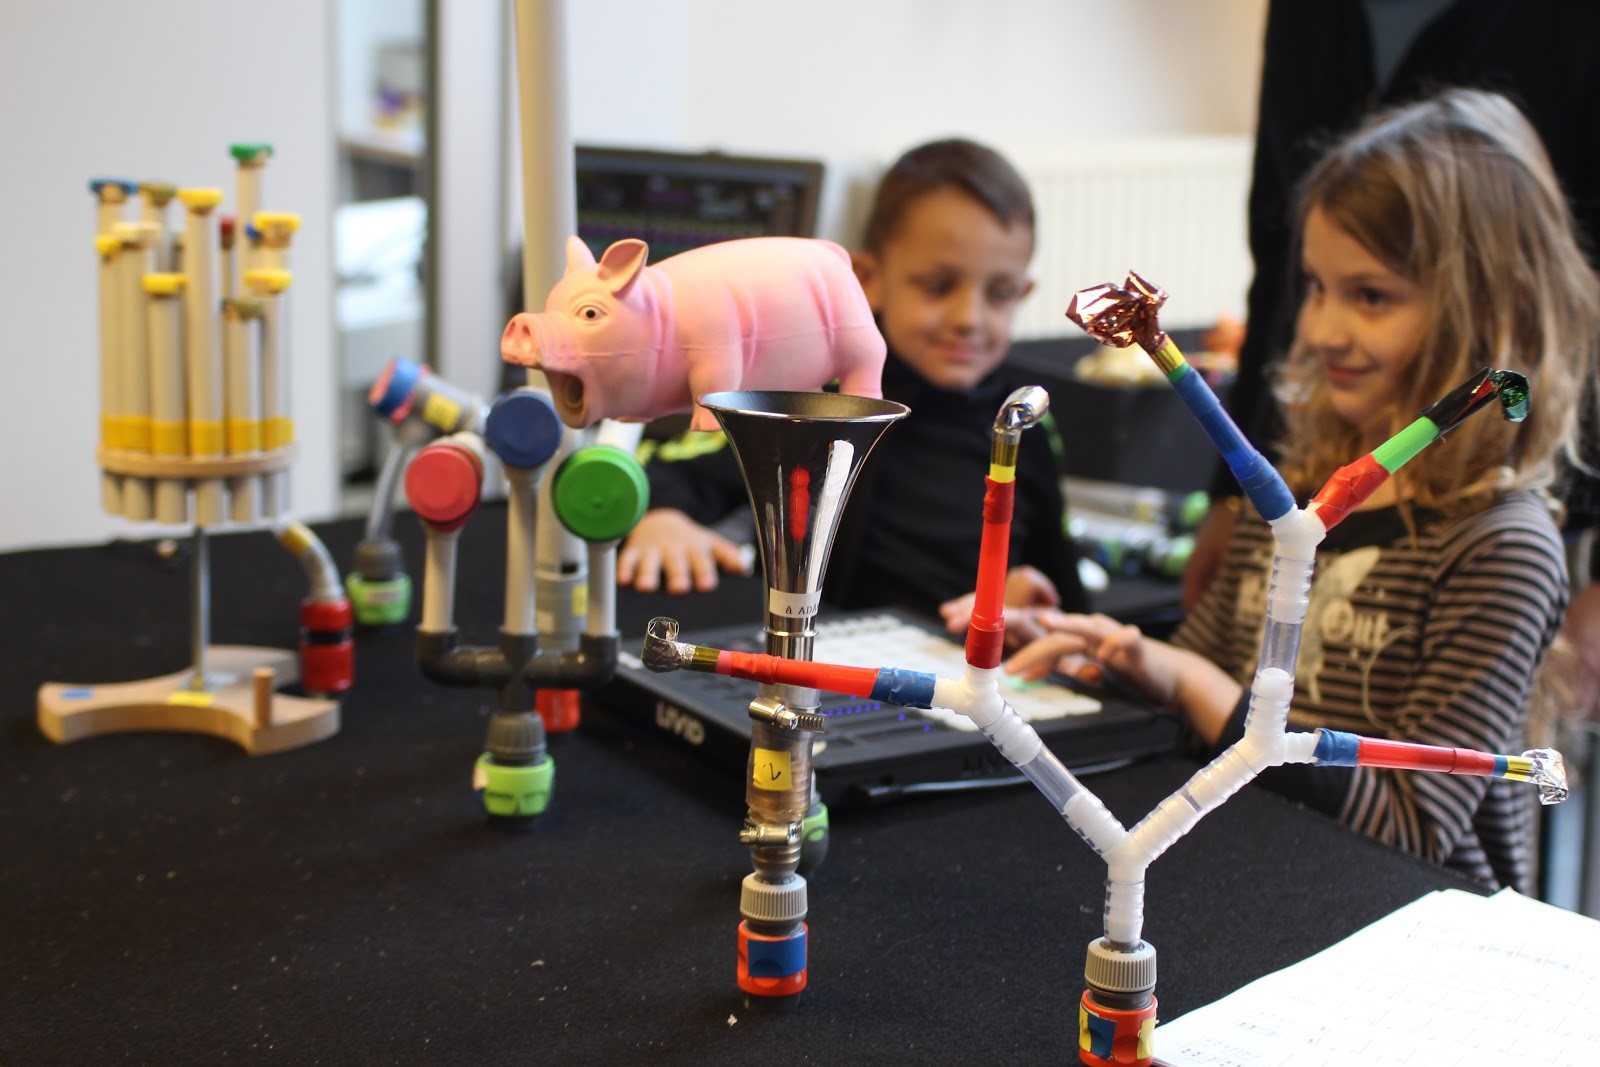
\includegraphics[width=6.5cm]{img/airmachine}
\label{fig:airmachine}
\end{wrapfigure}

\textit{Airmachine} est un instrument polyforme activé par l'air, soufflé ou aspiré périodiquement. Il s'agit d'un orgue contemporain sur lequel sont greffés différents types de prothèses sonores, toutes plus divertissantes les unes que les autres. Cet orgue humain et organique, accumulant instruments non accordés ou accordés, donne vie à des objets. C'est le rythme des poumons qui se donne à voir et à entendre.

En installation, en concert ou en atelier, Airmachine se décline donc sous différentes formes et offre des possibilités multiples en termes de médiation, notamment auprès du jeune public. Il s'agit avec cet instrument hors du commun de sensibiliser les enfants à l'écoute des sons, à la diversité de la création musicale contemporaine, de les familiariser avec le travail des compositeurs d'aujourd'hui, de développer leur créativité ou encore de leur transmettre le sens du collectif et de l'écoute.

À partir de la machine quelque peu loufoque d'Ondrèj Adámek, les jeunes sont amenés à réfléchir sur le rapport entre objet technique et création musicale, ainsi que sur les notions de soliste et d'orchestre, ou encore d'improvisation.\\

\noindent
\textbf{Publics :} scolaires dès 8 ans, périscolaires, adultes, familles.

\noindent
\textbf{A décliner en concert, installation, atelier scolaire ou tout public.}

\noindent
\textbf{Possibilité d'organiser un concert et/ou des ateliers en extérieur.}

\pagebreak

\section{Marathon créatif}
\label{app:marathon}

\begin{wrapfigure}{l}{7cm}
\centering
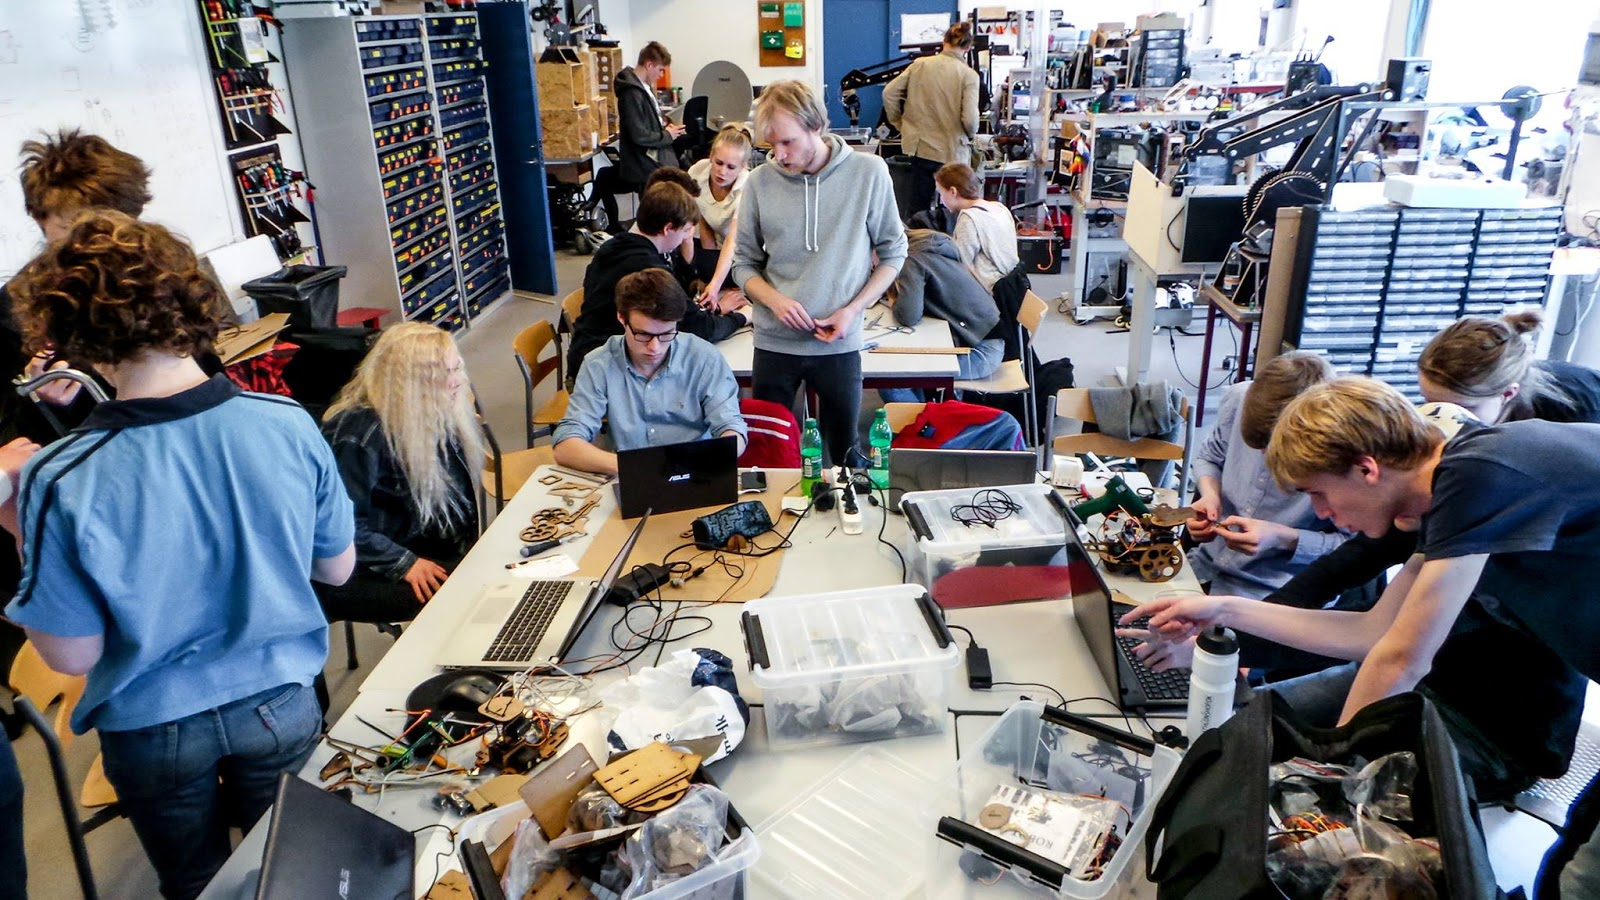
\includegraphics[width=6.5cm]{img/marathon}
\label{fig:marathon}
\end{wrapfigure}

Pendant 4 jours, le temps de la conférence SMC, des équipes pluridisciplinaires tout public (6-7 personnes par équipe), amateurs ou aguerris du monde de la musique, danse, de la technologie, du design etc., partageront une expérience de co-création. Sur un thème et avec des outils numériques et physiques mis à disposition, les participants travaillent ensemble pour explorer, tester les possibilités et produire une forme courte de création ou une installation, au carrefour de différentes approches.

Événement collaboratif pour imaginer les innovations qui pourront marquer la création sonore et visuelle de demain. Idée née d'une envie de combiner musique, danse et nouvelles technologies (motion capture, IA, VR, jeux vidéo, etc.) pour explorer de nouvelles façons d'écouter, de créer, jouer  et partager le son  avec des publics les plus variés possibles.

\textit{Objectif :}

\begin{itemize} 
\item Se familiariser aux méthodes et outils numériques de création musicale; 
\item Créer de façon ludique une performance  visuelle, sonore et/ou  chorégraphiée
\item Être concepteur et acteur d'une création collaborative.
\end{itemize}
     	 
\textit{Moyens :} lutherie physique et numérique mise à disposition des équipes. 
L'ensemble des outils de programmation et création conçus par Grame seront mis à disposition des participants (plateforme Faust IDE, Faust Audio Playground, Light Wall System, applis GameLan, etc.).\\

\noindent
\textbf{Publics :} dès 12 ans

\noindent
\textbf{Thème possible :} le jeu vidéo de demain 

\pagebreak

\section{Massages sonores}
\label{app:massage}

\begin{wrapfigure}{l}{7cm}
\centering
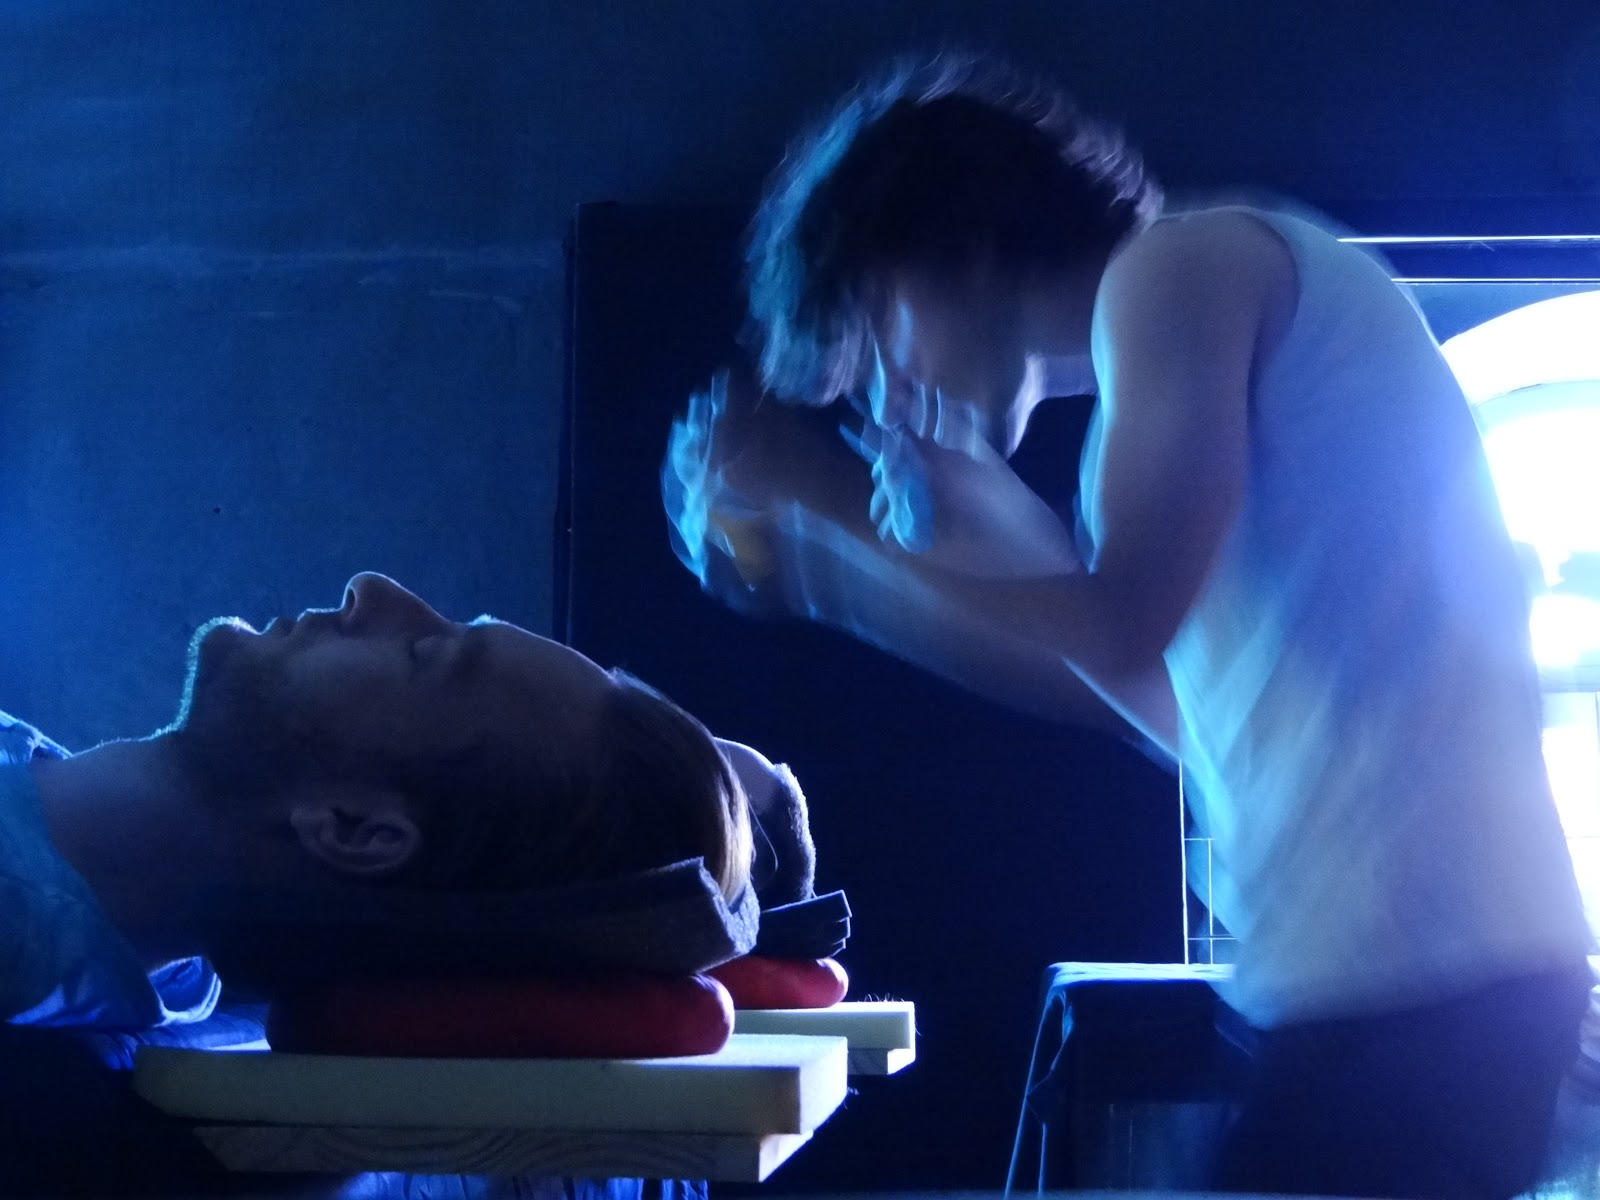
\includegraphics[width=6.5cm]{img/massage}
\label{fig:massage}
\end{wrapfigure}

Une écoute immersive d'une demi-heure, le temps de lâcher prise, de voyager intérieurement, de se détendre\dots La seule chose à faire, c'est laisser faire.

\textit{Massage sonore} est une installation dans laquelle le public entre dans un premier espace sonore, le paysage joué live par les performers, puis va être invité à s'allonger confortablement, de bien dégager l'espace proche de ses oreilles, puis de fermer les yeux. Les performers vont alors pouvoir détacher des parties du paysage sonore qu'ils génèrent pour venir les proposer dans le deuxième espace sonore, au creux de l'oreille, là où le micro-son n'a pas besoin d'amplification.

Le collectif NoMad fait le lien entre le paysage sonore et le massage aérien en proposant une expérience auditive dans laquelle l'auditeur est au centre du processus. Les musiciens réalisent un véritable massage audio sans aucun contact physique. Dans un attrape-rêves géant, chacun est invité à s'allonger les yeux fermés pour profiter d'une écoute sensationnelle.\\

\noindent
\textbf{Publics :} dès 10 ans

\noindent
\textbf{Par séance de 20 minutes, les participants s'allongent  dans des transats, puis se laisse aller à une écoute intérieure grâce à la vibration.}

\noindent
\textbf{Possibilité d'organiser les massages en extérieur.}

\pagebreak

\section{Vibes}
\label{app:vibes}

\begin{wrapfigure}{l}{7cm}
\centering
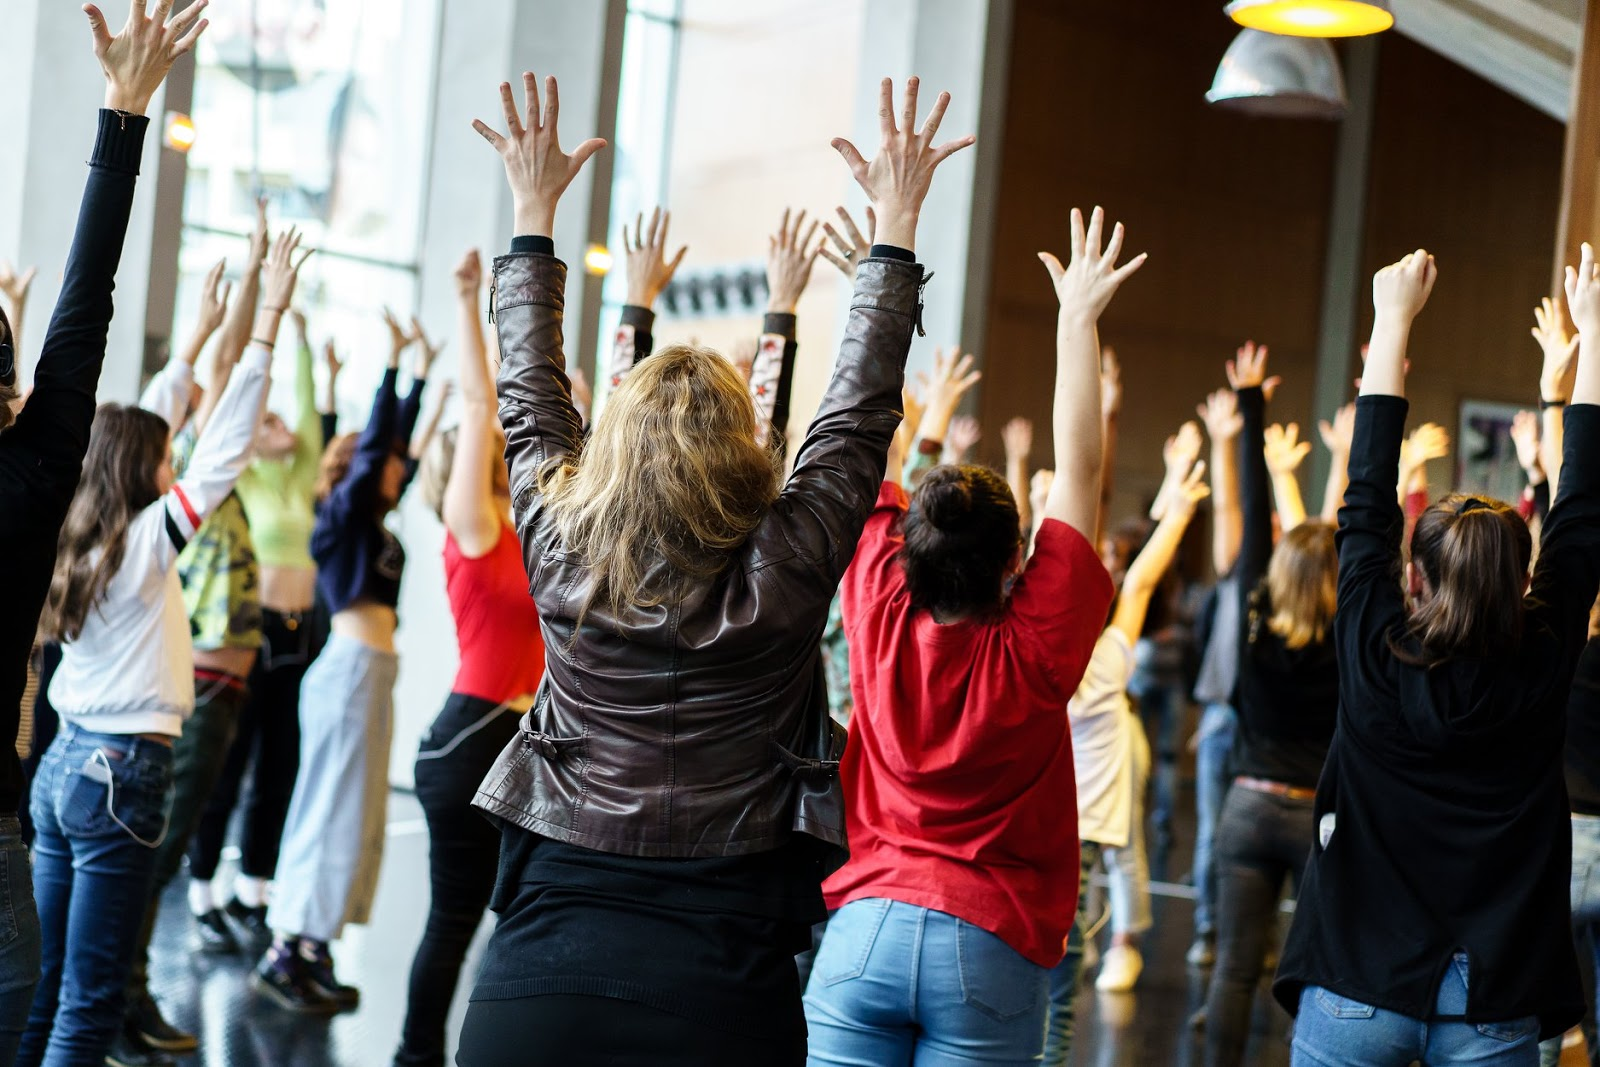
\includegraphics[width=6.5cm]{img/vibes}
\label{fig:vibes}
\end{wrapfigure}

À l'occasion de la conférence SMC, GRAME - CNCM propose un atelier de ``danse connectée'' nommé Vibes !

\textit{Qu'est-ce que Vibes ?}
Vibes est une application de rencontre chorégraphique et sonore. Elle permet à des utilisateurs de se rassembler pour partager un instant dansé dans un lieu donné ou dans différentes villes ou pays, au même moment. Équipés d'écouteurs, les danseurs improvisent ensemble leur danse grâce à l'audio-guidance d'un chorégraphe. Leurs mouvements et leurs déplacements dans l'espace influent sur la musique.

Pas besoin d'être danseur confirmé pour participer, seulement être disponible et motivé !\\

\noindent
\textbf{Publics :} dès 13 ans

\noindent
\textbf{45 min par session}

\noindent 
\textbf{Possibilité d'organiser l'action en extérieur.}

\pagebreak

\section{Veggie Orchestra}
\label{app:veggie}

\begin{wrapfigure}{l}{7cm}
\centering
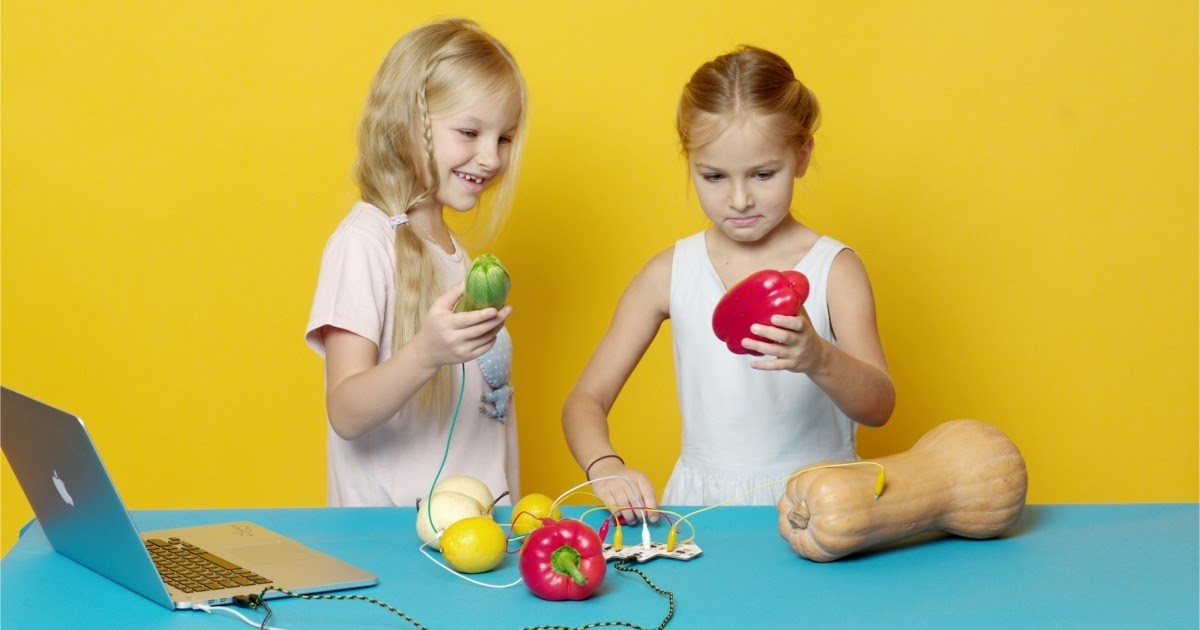
\includegraphics[width=6.5cm]{img/veggie}
\label{fig:veggie}
\end{wrapfigure}

A l'arrivée de l'été, on prend soin de vous en vous invitant à retrouver votre forme olympique ! Comment ? en vous proposant un menu rafraîchissant non seulement pour vos papilles, mais aussi pour vos oreilles ! Le studio Playtronica propose une performance live pour le moins inattendue : un concert de fruits et légumes de saison à déguster en famille.
 
Favorisant un rapport organique avec le son, décuplant la créativité et l'esprit DIY, Playtronica vous montrera à quel point tout peut devenir instrument de musique !
 
Concert suivi d'un \textbf{atelier de création sonore interactive} dès 6 ans.
 
Oubliez la flûte - essayez plutôt une tomate ! Atelier à expérimenter en famille, qui  bousculera votre vision de la  pratique conventionnelle de l'orchestre.
 
Atelier de création sonore interactive qui fera découvrir aux publics comment faire chanter les fruits, les couleurs ou même le corps. Une manière ludique et créative de faire attention à ce que les objets du quotidien veulent nous dire si on leur pose les bonnes questions.
 
Atelier animé par Playtronica, studio international regroupant ingénieur·e·s, musicien·ne·s, designer·euse·s, dédié à la création d'expériences sonores autour du rapport physique et tactile entre la musique et les objets quotidiens. Leurs ateliers originaux s'appuient sur un kit d'outils développés par la communauté internationale de makers.\\

\noindent
\textbf{Publics :} dès 6 ans

\noindent
\textbf{Possibilité d'organiser l'action en extérieur}

\end{document}
